%% LyX 2.2.2 created this file.  For more info, see http://www.lyx.org/.
%% Do not edit unless you really know what you are doing.
\documentclass[english]{article}
\usepackage{mathpazo}
\renewcommand{\sfdefault}{uop}
\usepackage[T1]{fontenc}
\usepackage[latin9]{inputenc}
\usepackage{geometry}
\geometry{verbose,lmargin=3cm,rmargin=3cm}
\usepackage{babel}
\usepackage{float}
\usepackage{booktabs}
\usepackage{url}
\usepackage{amsmath}
\usepackage{amsthm}
\usepackage{amssymb}
\usepackage{graphicx}
\usepackage[authoryear]{natbib}
\usepackage[unicode=true,pdfusetitle,
 bookmarks=true,bookmarksnumbered=false,bookmarksopen=false,
 breaklinks=false,pdfborder={0 0 1},backref=false,colorlinks=false]
 {hyperref}
\title{{\Large{}A Cost-benefit Analysis of R\&D and Patents: Evidence from China}\footnote{I am grateful to Mark Roberts for his insightful comments and continuing support. I acknowledge Jonathan Eaton, Paul Grieco, Daniel Grodzicki, Charles Murry, Michael Sposi, and Hylke Vandenbussche for their helpful comments. I would like to thank all the participants at the Industrial Organization Brownbag at Pennsylvania State University. Last but not least, I am indebted to Jie Zhang, Wenping Zheng, and Fuxin Zhai for their generosity to share the datasets with me.}}
\makeatletter

%%%%%%%%%%%%%%%%%%%%%%%%%%%%%% LyX specific LaTeX commands.
%% Because html converters don't know tabularnewline
\providecommand{\tabularnewline}{\\}

%%%%%%%%%%%%%%%%%%%%%%%%%%%%%% Textclass specific LaTeX commands.
  \theoremstyle{plain}
  \newtheorem{lem}{\protect\lemmaname}
\theoremstyle{plain}
\newtheorem{thm}{\protect\theoremname}

\makeatother

  \providecommand{\lemmaname}{Lemma}
\providecommand{\theoremname}{Theorem}

\begin{document}

\title{\Large{}Value of Patents and Dynamic R\&D Choice: Evidence from
China's High-tech Manufacturing Firms\footnote{I thank Jonathan Eaton, Mark Roberts, Paul Grieco, Daniel Goriedzicki, and all other participants in IO Brownbag at Penn State.}}

\author{Zhiyuan Chen\thanks{Department of Economics, Pennsylvania State University. Email: chenzhiyuan1224@gmail.com}}
\maketitle

\begin{abstract}
How much does the value of patents account for the payoff to the firm's
investment in R\&D? To answer the question, this paper develops a
model that includes dynamic R\&D investment, patents, and productivity
by treating patents as realized innovation and allowing the patents
affect the firm's profits directly. The dynamic model characterizes
linkages between the firm's continuous R\&D choice, patent applications,
and future revenue productivity and profits. This model allows me
to estimate the costs and long-run benefits of R\&D by measuring the
difference in expected firm value generated by investment in R\&D.
More importantly, this framework provide estimate of the patent value,
which reflects the impact of patenting system on the return to R\&D.
I estimate the model by using a combined data set of China's high-tech
manufacturing firms. The first-step estimations show that: First,
R\&D is an important factor in explaining the patent applications
and patent-R\&D elasticity decreases with firm's capital stock; Second,
patents have positive and significant impact on the firm's revenue
productivity. 

\textsl{Keywords:} dynamic R\&D investment;patenting system; patents;
productivity
\end{abstract}

\section{Introduction}

The patenting system is an important institutional arrangement to
stimulate private investment in research. Through the patenting system,
a firm holding patents gain profits directly from licensing the technology to other firms. For example, in 2016 the world's biggest chip-design firm, Qualcomm, earns one third of its revenue from the technology licensing division.\footnote{See \url{http://www.economist.com/news/business/21715705-its-biggest-customer-apple-suing-it-1bn-qualcomm-again-under-attack-living}}
However, the existing studies on estimating the return to R\&D often
take the patenting system as irrelevant and estimate the private return
to R\&D without identifying the effect of patenting system. These
approaches leave question on the importance of patenting system in
the payoffs to the R\&D investment unanswered. How much does the patenting
system account for the payoff to the firm investment in R\&D? What
is the value of patents? This paper attempts to answer these questions
by developing and estimating a dynamic model that links dynamic R\&D
choice, patents, and revenue productivity and profits. The most important
feature of this model is that it incorporates the impact of patenting
system in encouraging innovation investment by allowing the patents
affect the profit directly. 

Estimating the private return to R\&D has been an important topic
in related areas. Most of existing empirical literature build on the
framework by \citet{griliches1979issues}. In this framework, investment
in R\&D enables the firm to accumulate knowledge. The stock of knowledge
plays a similar role as physical capital, labor, and materials, which
enter into the production function of a firm. Thus the marginal product
of this knowledge stock provides a measure of return to the firm's
investment in R\&D. Another strand of literature focus on the firm's
optimal R\&D choice in a structural model setting \citep{Peters2016,Peters2017}.
This framework requires the researchers to estimate a dynamic model
of the firm's decision to invest in R\&D. The expected long-run payoff
to R\&D is obtained by rationalizing the observed discrete R\&D choice
by the firms in the data. The advantage of this framework is that
it allows the researchers to perform counterfactual analysis based
on the structural estimates. However, none of these frameworks has
taken the effect of patenting system explicitly into account when
consider the return to R\&D. Since the patenting system is designed
to encourage private investment in innovation, incorporating the impact
of patenting system in the model would give us a more complete understanding
on the payoffs to R\&D. 

In this article, I regard patents as an indicator for the realized
innovations and the creation of Intellectual Property Rights (IPRs
hereafter) by the firm. As a measure of successful innovation, patents
represent the production innovation and\textbackslash{}or process
innovation that increase the firm's productivity. As is pointed out
by \citet{crepon1998research}, it is the outcome of innovation rather
than the input of innovation that influences the productivity of a
firm. One problem here is that a firm is unlikely to file patent applications
when the IPRs protection is weak or the firm wants to hide the innovation
or the innovation is not patentable\footnote{For example, in 1892, Coca-Cola patented its original formula, but
after the formula changed, it was not patented again.}. To deal with this problem, in the model I take the efficiency of
research an development in producing patents as given. In other words,
the incentive of applying for patents is treated as exogenous\footnote{This approach is employed in many reduced-form models analyzing the
relationship between R\&D and patents. }. Therefore, the environment of the theoretical model is closer to
the high-tech industries in which the patenting law is enforced more
strictly and the possibility of hiding patents is not a major concern
in the model. In comparison, the creation of IPRs allows the firm
to earn profits through licensing the patents to other firms directly\footnote{As is the example of Qualcomm.}.
This type of return is directly related to the patenting system, which
is an important part of the return on the investment in R\&D. By separating
the return to patents to the profits obtained through increasing the
productivity, this study provides a deeper understanding on the payoffs
to R\&D investment. 

The model captures several important features of R\&D and patents.
First, the investment in R\&D affects the expected outcome of patents.
Different from the discrete choice framework, this model allows the
investment in R\&D to be continuous. With more investment in R\&D,
the firm the expected number of patents increases. Second, the patents
represent the realized innovations and affect the firm's revenue productivity
and short-run profits directly. To take potential heterogeneity of
patents into consideration, the marginal effect of different types
of patents are allowed to be distinct. Third, these effect will be
transmitted into the future periods and affect the firm's decision
to invest in R\&D and the long-run firm value. The fourth is there
is uncertainty surrounding the effect of patents on productivity.
Fifth, the cost of innovation is affected by a firm's previous experience
of investment in R\&D. 

The rest of this paper is organized as follows. Section 2 discusses
the existing frameworks of estimating the private return to R\&D investment.
Section 3 is the theoretical model. In Section 4, I introduce the
data this paper uses. The empirical strategy and estimation results
are presented in Section 5. Section 6 contains the counterfactual
analysis. Section 7 concludes.

\section{Existing Frameworks of Estimating the Private Return to R\&D Investment}

Quantifying the private return to R\&D investment is important in
explaining the firm's incentives to investment in R\&D. There are
two major approaches. The first approach is the knowledge stock approach
developed by \citet{griliches1979issues}. In this framework, the
investment in innovation by the firm creates knowledge stock, which
is similar to physical capital in the way that they enter into the
production function. The marginal product of knowledge stock is interpreted
as the return to investment in R\&D, which can be calculated as the
partial derivative of output with respect to the knowledge stock.
Because this framework treats the knowledge as a stock variable, it
faces same problems that researchers usually face when calculating
the stock of physical capital. First, it is difficult to estimate
the initial stock of knowledge for each firm in the sample. Second,
past expenditures on R\&D contribute to current knowledge stock with
a certain rate of depreciation. In practice, the depreciation rate
is often assumed to be constant across different firms and periods.
This may cause serious bias to the estimation of knowledge stock.
Despite of these limitations, this framework is extended in various
ways\footnote{\citet{Hall2010} provides a recent review of the empirical evidence
on estimating the return to R\&D investment.}. The most important extension related to this paper is the econometric
framework proposed by \citet{crepon1998research}(CDM hereafter).
In the CDM framework, it is the expected output of R\&D investment
(measured by patent applications or innovative sales) that affects
the productivity rather than the R\&D investment itself. However,
their framework provides no estimate for the return to R\&D or the
value of patents. 

Different from the knowledge stock approach, the endogenous productivity
approach incorporates R\&D in the process of productivity evolution
as implemented by \citet{Awetal.2011} and \citet{Doraszelski2013}.
By this approach, the firm's productivity is modeled as a Markov process.
The conditional mean of the productivity in next period is affected
by the R\&D investment in the current period. This approach avoids
the problem of calculating the knowledge stock for each firm by capturing
the impact of distant past R\&D spending in the productivity in the
last period. More importantly, this framework adds uncertainty to
the evolution of productivity; a random shock to current productivity
will be transmitted to future productivity. In this formulation, this
framework allows for different productivity levels even for firms
with identical historical path of R\&D expenditures. Because endogenous
productivity approach treats the R\&D investment as innovation outcome
that affects the productivity directly, this approach does not explicitly
consider the transformation of R\&D into realized innovation. One
important recent extension of this framework is by \citet{Peters2017}(PRVF
hereafter). In PRVF, the firm invests in R\&D in order to realize
product or process innovation in the future. When an innovation (either
process or product) is realized, it alters the distribution of future
productivity, which ultimately influence the expected future profits.
This model is in the same spirit of CDM in the sense that only the
realized innovation affects the firm profits through influencing the
distribution of the future productivity.

The model in this paper is based on the PRVF and CDM, but the model
differs from these frameworks in following two aspects. First, in
this model the investment in R\&D increases the production of patents
that affect the firm's future profits through increasing the firm's
future productivity and profits from licensing patents to other firms.
It is different from PRVF since the patents can affect the firm's
profits directly while the realized innovation can only influence
the profits through the productivity. It is also different from CDM
because in their econometric framework patents are only treated as
realized innovation rather than intellectual property rights to the
firm. Second, in this paper, both the extensive margin and intensive
margin of R\&D is considered. The zero investment in R\&D is rationalized
as a corner solution to the firm's dynamic programming problem and
different counts of patents can be explained by different levels of
R\&D expenditures. This is an extension of PRVF since they only considered
the discrete choice of R\&D investment, which only captures the extensive
margin of R\&D investment. While CDM consider the intensive and extensive
margin of R\&D investment, their concern is mainly related to the
econometric issue related to the sample selection problem caused by
the corner solution.

\section{Theoretical Model}

In this section, I develop a theoretical model of a firm's dynamic
R\&D choice and production of patents. This model is built on the
PRVF model. In the PRVF model, a firm's R\&D decision changes the
probability of realizing product or process innovations. The realized
innovations affect the firm's future productivity and expected profits.
A firm chooses whether to invest in R\&D or not to maximize its net
profits. Different from their model, I allow R\&D choice to be continuous
and specify production functions for the patents. Then I regard patents
outcome as the realized product or process innovations which also
enter the evolution equation of the productivity. More importantly,
I allow patents to affect the profits directly, which captures the
impact of patent licensing on the profits. 

As in PRVF, the model comprises of four structural parts. The first
part is the firm's patents production function that links the expected
number of patents with firms investment in R\&D. The second component
is the cost function for investment in R\&D, which is influenced by
the previous experience in R\&D. The third component of the model
links a firm's patent activities with the process of productivity
evolution, in which patents alter the probability distribution of
the firm's future productivity. I also assume that patents can affect
the firm's profits directly through licensing the technology to other
firms. The last component of the model is a profit function specifying
the relationship between productivity, patents and profits. In equilibrium,
a firm will optimally choose the level of investment in R\&D to maximize
its expected profits. Figure 1 provides an overview of the model.
In the remainder of this section I will discuss each part of the model
in more detail.
\begin{center}
\begin{figure}[h!]
\caption{An overview of the model}
\label{F1}

\begin{centering}
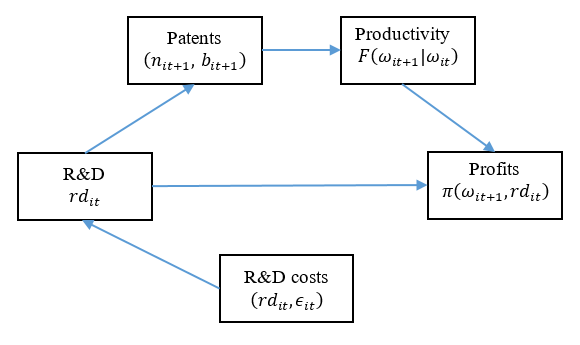
\includegraphics[width=1\textwidth]{Overview.PNG}
\par\end{centering}
\end{figure}
\par\end{center}

\subsection{Patents production function and R\&D costs}

\paragraph{Production function for patents.}

The key assumption of the model is that R\&D is an input of innovation
and cannot affect the productivity process directly. Instead, the
patenting activities, which represent the output of innovation, will
alter the distribution of future productivity. This setup is the same
as \citet{crepon1998research}. Let $rd_{it}$ be the log of firm
$i$'s investment in R\&D in period $t$ when the R\&D investment
is greater than zero, and $rd_{it}=0$ when the R\&D investment is
zero\footnote{To preserve the relative magnitude of investment in R\&D, I normalize
the investment in R\&D in the dataset such that it is not contained
in the interval of $\left(0,\,1\right]$.}. Denote $N_{it+1}$ and $B_{it+1}$as the number of counts for invention
patents applications and utility patent applications, respectively.
Following \citet{Hausman1984}, I model the production of patents
by following two moment conditions:
\begin{align}
\bar{N}_{it+1}=\mathbb{E}\left(N_{it+1}|rd_{it}\right) & =\exp\left(\alpha_{0}+\beta_{0}rd_{it}+\gamma_{0}Z_{it}\times rd_{it}\right)\label{invp}\\
\bar{B}_{it+1}=\mathbb{E}\left(B_{it+1}|rd_{it}\right) & =\exp\left(\alpha_{1}+\beta_{1}rd_{it}+\gamma_{1}Z_{it}\times rd_{it}\right)\label{utip}
\end{align}
Here I do not make further assumption on the distribution of the patents
outcome in building the theoretical model. But in the estimation,
I will make additional assumption for the distribution of patents
to take the counting feature of patents into consideration. Note that
$rd_{it}$ affects the production of invention patents and utility
patents through different parameters but given $\left(\alpha_{j},\beta_{j}\right)$
($j\in\left\{ 0,1\right\} $) , $\bar{N}_{it+1}$ and $\bar{B}_{it+1}$
are correlated since they are both affected by investment in R\&D.
One drawback of this approach of modeling the relationship between
patents and investment in R\&D is that it regards the incentives of
applying patents as exogenous. However, the number of patent applications
filed by the firm is an endogenous choice made by the firm. Factors
such as patent law and the length of examination time will affect
the firm's incentive to apply patents. \citet{Lei2012} find that
Chinese firms tend to break up their inventions in order to file more
patent applications to receive more patent subsidies. This shows that
firms have discretion over the number of patent application for a
given number of claims. To account for potential differences in the
efficiency of research and development and the propensity to apply
for patents, I also include interactions between firm's other characteristics
such as age, size, and industry and investment in R\&D, which is denoted
as $Z_{it}\times rd_{it}$. Hence $\gamma_{0}$ and $\gamma_{1}$
represent the heterogeneity in the efficiency of undertaking investment
in R\&D. I also denote the logs of the two different kinds of patents
as $\bar{n}_{it+1}$ and $\bar{b}_{it+1}$, respectively; their roles
in the model will be explained later.
\begin{center}
\begin{figure}[H]
\caption{Different levels of R\&D and average number of patents}

\begin{centering}
\begin{tabular}{c}
\includegraphics[scale=0.8]{\string"E:/Data/Patents/rdppsub/preliminary statistics/graphs/PatentsVariationLags\string".pdf}\tabularnewline
\end{tabular}
\par\end{centering}
{\small{}Note: The classification of levels of investment in R\&D
is: 0: $rd_{it-1}=0$1: $rd_{it-1}\in\left(0,\,3\right]$; 2: $rd_{it-1}\in\left(3,\,6\right]$;
3: $rd_{it-1}\in\left(6,\,9\right]$; 4: $rd_{it-1}>9$. }{\small \par}
\end{figure}
\par\end{center}

I treat the firm's R\&D decision as a continuous choice variable for
following reason. In my data, I observe substantial differences in
the number of patents applications for different levels of R\&D expenditures.
In Figure 2, I plot the average number of patents against different
levels of investment in R\&D for all the three different types of
patents using my data set. As we can see, when the investment in R\&D
increases, the average number of increases more significantly for
invention patents and invention patents. But the change of the average
number of design patents is relatively mild as the investment in R\&D
increases. This implies that modeling a discrete choice of investment
in R\&D is not sufficient to explain the variation in the patents.
Using discrete choice to model the R\&D decision will lead to a great
loss of information on the linkage between investment in R\&D and
patent applications. Treating R\&D choice as a continuous variable
allows me to connect different numbers of patent applications with
the variations in R\&D expenditures. The issue of using R\&D spending
is that it may introduce more measurement error into the model. However,
I choose to treat the measurement error as additive and independent
of the real expenditures on R\&D. Thus the estimator of the coefficients
on R\&D are still consistent. 

\paragraph{R\&D costs. }

Following PRVF, I assume that firms undertaking R\&D activities are
heterogenous in their innovation costs\footnote{This may be caused by the managerial efficiency, the efficiency of
R\&D labs, the innovation ability of research scientists, and nature
of innovation projects on hand. }. In PVRF, the innovation cost is assumed to be dependent on prior
R\&D experience and current capital stock. While in PVR, a firm's
R\&D cost is determined by previous R\&D experience and its financial
strength. Previous R\&D experience is an important determinant of
the R\&D costs because it allows the firm to rely on past expertise
from prior projects. Therefore we expect that a firm that participate
in R\&D activities continuously over time is likely to perform R\&D
at lower costs. Different from PRVF and PRV, I treat R\&D decision
as a continuous choice. When investing in R\&D, the costs of R\&D
for each firm is given as
\begin{equation}
C_{it}=\mathbb{I}\left(rd_{it}>0\right)\exp\left(rd_{it}\right)\epsilon_{it},\label{rd cost}
\end{equation}
where $\epsilon_{it}$ is a cost shock known by the firm but not by
the econometrician and follows an i.i.d exponential distribution:
\[
\epsilon_{it}\sim\text{Exp}\left\{ \kappa^{m}\times\mathbb{I}\left(rd_{it}>0\right)+\kappa^{s}\times\left[1-\mathbb{I}\left(rd_{it}>0\right)\right]\right\} 
\]
I also assume that the firm knows $\kappa^{s}$ and $\kappa^{m}$.
According to the specification in (\ref{rd cost}), a firm with prior
R\&D experience has to pay a maintenance cost and new investment which
sum up to $\exp\left(\kappa^{m}+rd_{it}\right)$ and a firm without
past experience in undertaking R\&D has to pay a startup cost and
new investment in R\&D which add up to $\exp\left(\kappa^{s}+rd_{it}\right)$.\footnote{This formulation is different from \citet{Maican.etal.2017}. In their
model, they assume that there is a fixed cost for innovation and the
fixed cost is affected by the firm's prior experience in R\&D activities.} A firm knows its innovation cost before they make the R\&D choice.
Also note that whether investment in R\&D or not shifts the mean of
the distribution of the R\&D costs in the future.

\subsection{Firm's short-run profits}

I assume that firm's short-run marginal cost is affected by capital
stock, age, and unobserved production efficiency and is specified
as following:
\begin{equation}
mc_{it}=\beta_{c}+\beta_{k}k_{it}+\beta_{a}a_{it}+\beta_{m}p_{mt}+\beta_{l}p_{lt}-\phi_{it},
\end{equation}
where $mc_{it}$ is the log of marginal cost, $k_{it}$ is the log
of the firm's capital stock, $a_{it}$ is the firm age, and $p_{mt}$
and $p_{lt}$ are prices for intermediate materials and labor that
all firm faces in period $t$, separately. $k_{it}$ is treated as
a fixed factor in the short-run. $\phi_{it}$ captures differences
in technological efficiency or managerial ability or input quality,
which are known by the firm but not by the econometrician. $\phi_{it}$
is also known as the physical productivity that is different from
the revenue productivity to be defined later. 

The demand function is derived from the Dixit-Stiglitz demand system
and is of constant elasticity. For firm $i$ in year $t$, the demand
for the firm's product $q_{it}$ is given by 
\begin{equation}
q_{it}=Q_{t}\left(\frac{p_{it}}{P_{t}}\right)^{\theta}\exp\left(\lambda_{it}\right)=\Lambda_{t}\left(p_{it}\right)^{\theta}\exp\left(\lambda_{it}\right),
\end{equation}
where $Q_{t}$ is the aggregate industry output in period and $P_{t}$
is the industrial price index. $p_{it}$ and $\lambda_{it}$ are the
product price and demand shifter, respectively. I combine the industry-level
variable into $\Lambda_{t}$. The demand factor $\lambda_{it}$ is
unobservable to the econometrician but is known by the firm. The elasticity
of demand is $\theta<-1$, which is negative and assumed to be constant
for all firms within the same industry. Firms operating in the market
maximizes its short-run profit by equalizing its marginal cost with
the marginal revenue, the first-order condition gives the pricing
rule as follows:
\begin{equation}
p_{it}=\frac{\theta}{1+\theta}\exp\left(mc_{it}\right)\label{pricing rule}
\end{equation}
Then the log of short-run revenue $r_{it}$ from selling products
can be represented as:
\begin{align}
r_{it} & =\left(1+\theta\right)\ln\left(\frac{\theta}{1+\theta}\right)+\ln\Lambda_{t}\label{revenue}\\
 & +\left(1+\theta\right)\left(\beta_{c}+\beta_{k}k_{it}+\beta_{a}a_{it}+\beta_{m}p_{mt}+\beta_{l}p_{lt}-\omega_{it}\right)\nonumber 
\end{align}
where $\omega_{it}$ represents the revenue productivity and is defined
as 
\[
\omega_{it}\equiv\phi_{it}-\frac{\lambda_{it}}{1+\theta}
\]
As PRVF point out, the revenue productivity captures both the impact
of production efficiency ($\phi_{it}$) and the demand shifter ($\lambda_{it}$).
Given capital stock and firm age, firm heterogeneity in the revenue
is driven by differences in the revenue productivity. Because $\theta$
enters into the revenue productivity ans is assumed to be constant
within the same industry, the estimates of revenue productivity are
likely to reflect differences in markups. To separate the revenue
productivity into $\phi_{it}$, $\lambda_{it}$, and markups, we need
information on quantity and price of the firms. For the purpose of
this study, I only quantity the effect of $\omega_{it}$ on firm sales
and profits. Combining the pricing rule (\ref{pricing rule}) and
revenue equation (\ref{revenue}), we obtain a simple relationship
between firm's short-run profits from producing products and revenue
productivity:
\begin{align}
\pi_{0}\left(\omega_{it}\right) & =-\frac{1}{\theta}\exp\left(r_{it}\right)\label{pi0(10)}
\end{align}

Different from existing frameworks, I consider the profits directly
from patent applications. These profits are usually obtained by licensing
patents to other firms, which differs from the profits from selling
products in the sense that the firm rents technology to other firms.
To model the direct impact of patents on the firm profits, I assume
that the profits from filing patent applications are given by:
\begin{equation}
\pi_{1}\left(n_{it},b_{it}\right)=\eta\left(n_{it}+b_{it}\right)\label{pi_1}
\end{equation}
The linearity assumption is mainly made for simplicity; $\eta$ captures
the average marginal net benefits through patent licensing for invention
and utility patents, separately\footnote{The assumption that the marginal net benefits for invention and utility
patents is the same comes mainly from the the problem of identification.
Note that we model the production of invention patents and utility
patents in a way such that the log of expected patents are linear
in log of investment in R\&D. In this case, we can write $\pi_{1}$
as a function of the investment in R\&D in previous period and identify
a weighted sum of the coefficient. }. We expect that $\eta$ to be increasing when there is a strengthening
of patent law or there is a reduction in patent application fees.
Therefore the total profits of the firm is given by
\begin{equation}
\pi\left(\omega_{it},\,n_{it},b_{it}\right)=\pi_{0}\left(\omega_{it}\right)+\pi_{1}\left(n_{it},b_{it}\right)\label{pi}
\end{equation}
The ratio of $\pi_{1}$ to $\pi_{0}$ is of central importance in
the model because it captures the relative importance of patent licensing
in explaining the payoff to R\&D investment. For the convenience of
discussion, let's define
\begin{equation}
\chi\left(\omega_{it},\,n_{it},\,b_{it}\right)\equiv\frac{\pi_{1}\left(n_{it},b_{it}\right)}{\pi_{0}\left(\omega_{it}\right)}
\end{equation}
Note that $\chi\left(\omega_{it},\,n_{it},b_{it}\right)$ is the ratio
of one-period profits from licensing patents to that from product
sales. A larger $\chi$ implies: (1) the firm's leading position in
the innovation race; (2) the protection of IPRs is relatively strong.
In contrast, when $\chi\left(\omega_{it},\,n_{it},b_{it}\right)$
is small, the firm gain its profits mainly from upgrading its own
technology instead of renting technology to other firms. In the PRVF
and\textbackslash{}or CDM, $\chi\left(\omega_{it},\,n_{it},b_{it}\right)$
is always zero because all the benefits of R\&D are attributed to
the increasing of productivity which ultimately raises the profits.
Since we have assumed that $n_{it}$ and $b_{it}$ is a deterministic
function of the prior-period investment in R\&D, we can write $\chi$
as $\chi\left(\omega_{it},\,rd_{it-1}\right)$. $\chi$ is usually
not observable in the firm-level data, but we can infer the upper
bound or lower bound of it using the information available in the
data since the profits from patent licensing to other firms is a part
of revenue from other activities. If we check the ratio of profits
from major activities (sales) to the profits from other activities,
a positive (negative) ratio gives us information on the upper (lower)
bound of $\chi$. In the data used in the paper, the average of this
number is around 0.09 with a variation around 13.74. It also varies
greatly across industries. The means of the ratios for the high-tech
industries are: electrical machinery (.173), pharmaceutical manufacturing
(.135), special equipment (-0.365), and electronics (-0.083). As we
will see shortly, estimating this model enables me to back out $\chi$
that gives us information on the value of patents.

\subsection{Endogenous productivity}

As a measure of realized innovation, patents can endogenously alter
the evolution of productivity, and eventually, the profits over time.
However, only invention patents and utility patents are assumed to
be able to alter the productivity process because design patents are
of the lowest quality and is not a representative indicator for either
product or process innovation. In fact, design patents are particularly
related to the design of outlook of the firm's products\footnote{According to Article 22 of the Patent Law of the P.R.C.: any invention
or utility model for which patent right may be granted must possess
novelty, inventiveness and practical applicability. In comparison,
the requirement for the approving of design patents is in Article
24 of the Patent Law of the P.R.C as \textquotedblleft \dots \dots must
not be identical with or similar to any design which, before the date
of filing, has been publicly disclosed in publications in the country
or abroad or has been publicly used in the country, and must not collide
with any legal prior rights obtained by any other person.\textquotedblright{}
This will be more clear when we discuss the estimation results of
patents production function.}. I expect that it will not influence the revenue productivity significantly. 

To simplify the structure of the expectation, I follow \citet{crepon1998research}
and assume that only the outcome of innovation affects the productivity
process. Let $\omega_{it}$ be the revenue productivity of firm $i$
in period $t$. The patent-productivity linkage is modeled by the
CDF $F\left(\omega_{it+1}|\omega_{it},\,n_{it+1},b_{it+1}\right)$,
where the distribution of future productivity is affected by a firm's
past productivity and logs of the current realizations of invention
patents ($n_{it+1}$) and utility patents ($b_{it+1}$). This formulation
also captures the uncertainty in the benefits of innovation facing
the firms. This aspect of uncertainty is different from the uncertainty
of producing patents because it happens after the realization of patents.
Specifically, the evolution equation of firm productivity is as following:
\begin{equation}
\omega_{it+1}=h\left(\omega_{it},\,n_{it+1},\,b_{it+1}\right)+\varepsilon_{it+1}
\end{equation}
where $h\left(\omega_{it},\,n_{it+1},\,b_{it+1}\right)$ is the conditional
mean of future productivity and $\varepsilon_{it+1}$ is an i.i.d
stochastic shock normally distributed with zero mean and variance
$\sigma_{\varepsilon}^{2}$. As pointed out by PRVF, this formulation
assumes that (1) a firm's productivity is persistent over time; (2)
innovation outcomes systematically shift the mean of the distribution
of future productivity, and (3) productivity change is affected by
stochastic shocks $\varepsilon_{it+1}$. More importantly, rather
than linking future productivity directly to R\&D as in \citet{Awetal.2011}
and \citet{Doraszelski2013}, expected future productivity evolves
only when the firm produces any invention or utility patents. To account
for the difference between invention patents and utility patents in
affecting the firm's future productivity, I also allow that $\partial\omega_{it+1}/\partial n_{it+1}$
and $\partial\omega_{it+1}/\partial b_{it+1}$ to be different in
the estimation. 

\subsection{Equilibrium R\&D choice}

I close this model by considering the firm's optimal choice of investment
in R\&D to maximize its profits. Assume that at the start of period
$t$, the firm is able to observe its current revenue productivity
$\omega_{it}$ and the short run profit function $\pi\left(\omega_{it},\,n_{it},\,b_{it}\right)$
, the patents production equation, and the productivity evolution
process. To link the R\&D choice to the patents that enter into the
profit function. I replace the $n_{it}$ and $b_{it}$ to be the expected
number $\bar{n}_{it}$ and $\bar{b}_{it}$, respectively. By (\ref{invp})
and (\ref{utip}) the expected number of patent applications is a
function of prior-period R\&D investment, we can write the profit
as a function of profits and past R\&D experience, which is $\pi\left(\omega_{it},\,rd_{it-1}\right)$.
The evolution of the firm's state $\Omega_{it}=\left(\omega_{it},\,rd_{it-1}\right)$
is affected by the firm's decision to undertake R\&D, $rd_{it}$.
A firm chooses investment in R\&D to maximize its firm value. I will
omit the subscripts of firm and year whenever no confusion arises.
Let $\delta$ be the discounting factor, the firm's problem is given
as:
\begin{equation}
V\left(\Omega,\,\epsilon\right)=\pi\left(\omega,\,rd_{-1}\right)+\max_{rd\geq0}\left\{ \delta EV\left(\Omega,\epsilon,rd\right)-\mathbb{I}\left(rd>0\right)\exp\left(rd\right)\epsilon\right\} \label{firm_vf}
\end{equation}
where the expected value of the firm in next period is 
\[
EV\left(\Omega,\epsilon,\,rd\right)=\int_{\Omega'}\int_{\epsilon'}V\left(\Omega',\,\epsilon'\right)p\left(d\Omega',\,d\epsilon'|\Omega,\,\epsilon,\,rd\right)
\]
where $p\left(d\Omega',\,d\epsilon'|\Omega,\,\epsilon,\,rd\right)$
is the conditional probability density function. Following the conditional
assumption introduced by \citet{Rust1987}, I assume that 
\begin{equation}
p\left(d\Omega',\,d\epsilon'|\Omega,\,\epsilon,\,rd\right)=p\left(d\Omega'|\Omega,\,rd\right)p\left(d\epsilon'|\Omega'\right)\label{CI}
\end{equation}

According to Equation (\ref{firm_vf}), a firm chooses the level of
investment in R\&D to maximize its firm value. Because the cost function
of R\&D is not continuous at zero, the model can also rationalize
the corner solution. The model incorporates both extensive margin
and the intensive margin of R\&D expenditures. Therefore the model
extends the frameworks of CDM and PRVF in the sense that it treats
R\&D choice as a continuous variable and is able to reconcile the
fact that a large portion of the firms do not participate in R\&D
activities. In summary, the model endogenizes the firm's choice to
undertake R\&D investment as a result of maximizing the long-run firm
value.

One important aspect of this problem is the continuous choice of investment
in R\&D when a firm decides to invest in R\&D. Note that for $rd>0$,
a firm has to choose the R\&D expenditures such that it maximizes
the firm value; the optimal choice of investment in R\&D is:
\begin{equation}
rd^{*}=\arg\max_{rd>0}\left\{ \delta EV\left(\Omega,\epsilon,rd\right)-\exp\left(rd\right)\epsilon\right\} 
\end{equation}
Taking derivative with respect to $rd$ , the first-order condition
and envelop condition can be combined into following Euler equation:
\begin{equation}
\delta\mathbb{E}\frac{\partial\pi\left(\omega',\,rd\right)}{\partial rd^{*}}=\exp\left(rd^{*}\right)\epsilon\label{Euler}
\end{equation}
This equation characterizes the continuous part of the choice in investment.
The optimal choice of investment in R\&D must satisfy the equation
above. Following Lemma justifies the existence of a threshold of $\epsilon$
below which the firm chooses to invest in R\&D. 
\begin{lem}
Under the conditional independence assumption, for any $\Omega$ there
exists $\bar{\epsilon}$ such that the firm chooses to invest in R\&D
when $\epsilon<\bar{\epsilon}$.
\end{lem}
\begin{proof}
First, define $EV^{1}\left(\Omega,\,\epsilon\right)=\max_{rd>0}\left\{ \delta EV\left(\Omega,\epsilon,rd\right)-\exp\left(rd\right)\epsilon\right\} $
and $EV^{0}\left(\Omega,\,\epsilon\right)=\delta EV\left(\Omega,\epsilon,0\right)$.
A firm will have positive investment in R\&D if and only if$EV^{1}\left(\Omega,\,\epsilon\right)-EV^{0}\left(\Omega,\,\epsilon\right)>0$.
Note that $EV^{1}\left(\Omega,\,\epsilon\right)$ is decreasing in
$\epsilon$. By the assumption of (\ref{CI}), $EV^{0}\left(\Omega,\,\epsilon\right)$
is independent of $\epsilon$ and can be written as $EV^{0}\left(\Omega\right)$.
As $\epsilon\rightarrow0$, $EV^{1}\left(\Omega,\,\epsilon\right)>EV^{0}\left(\Omega\right)$
and as $\epsilon\rightarrow\infty$, $EV^{1}\left(\Omega,\,\epsilon\right)<EV^{0}\left(\Omega\right)$.
By the mean value theorem, there exists a $\bar{\epsilon}$ such that
$EV^{1}\left(\Omega,\,\bar{\epsilon}\right)=EV^{0}\left(\Omega\right)$
and $EV^{1}\left(\Omega,\,\epsilon\right)>EV^{0}\left(\Omega\right)$
when $\epsilon>\bar{\epsilon}$.
\end{proof}
The theorem below provides the relationship between the choice of
$rd$ and $\epsilon$ conditional on the state $\Omega$. 
\begin{thm}
Conditional on $\Omega$, if $\epsilon<\bar{\epsilon}$, the optimal
choice of investment in R\&D is decreasing in $\epsilon$. 
\end{thm}
\begin{proof}
Consider two different $\epsilon^{1}$ and $\epsilon^{2}$, which
are all smaller than $\bar{\epsilon}$. Denote the corresponding optimal
investment in R\&D as $rd^{1}$ and $rd^{2}$. Without loss of generality,
assume that $\epsilon^{1}<\epsilon^{2}$. Then the Euler equation
implies that 
\begin{align*}
\delta\mathbb{E}\frac{\partial\pi\left(\omega',\,rd\right)}{\partial rd^{1}} & =\exp\left(rd^{1}\right)\epsilon^{1}\\
\delta\mathbb{E}\frac{\partial\pi\left(\omega',\,rd\right)}{\partial rd^{2}} & =\exp\left(rd^{2}\right)\epsilon^{2}
\end{align*}
Now suppose that $rd^{1}\leq rd^{2}$, then this implies that $\delta\mathbb{E}\frac{\partial\pi\left(\omega',\,rd\right)}{\partial rd^{2}}>\delta\mathbb{E}\frac{\partial\pi\left(\omega',\,rd\right)}{\partial rd^{1}}=\exp\left(rd^{1}\right)\epsilon^{1}$.
But this violates that $rd^{1}$ is an optimal solution for $\epsilon^{1}$.
Therefore it must be that $rd^{1}>rd^{2}$. 
\end{proof}
In the next section, I will introduce the dataset this study uses.
Based on the dataset, I will develop empirical models to estimate
each component of the model.

\section{Data}

\subsection{Data sources}

\paragraph{Firm-level production data. }

The first data set is the data on Chinese manufacturing firms from
2001 to 2007 complied by China's National Bureau of Statistics (CNBS
hereafter). This data set is widely used in studies on Chinese firms.
This data set includes all Chinese State Owned Enterprises (SOEs hereafter)
and non-SOEs with annual sales no less than five million \textit{Renminbi}
(equivalent to about 700,000 US dollars). These firms accounts for
98\% of the manufacturing exports. This data set contains all the
information of the firm's major accounting sheets, which includes
more than 100 financial variables. Specifically, it includes firm
sales, number of employees, material input, fixed assets, R\&D expenditures,
and firm characteristics like firm age and its industrial code. In
summary, this rich data set provide the information on the firm-level
production activities.

\paragraph{Patent data.}

This study also employs the patents database collected by the State
Intellectual Property Office (henceforth SIPO) of China. It contains
all the patents that are applied and certified in mainland China.
Specifically, for each patent the database has the information on
its type (invention, utility model, and design), owner, application
time, certification time, agent of application, abstract, location,
and expiration time during 1985 and 2012. But it should be noted that
there is no information on citations for patents in the database,
which makes it difficult to measure the patents quality directly.

\paragraph{Final combined database.}

For the purpose of this study, I merge these two data sets using the
firm name. Table 1 shows aggregate information on the number of patents
for the combined database. The aggregate number of invention patents
and utility patents show a strong increasing trend over the sample
period. One important concern on using the combined data set is the
efficiency of matching between these two data sets. To evaluate the
matching efficiency, in the last row of Table 1, I show the percentage
of the total number of invention patents in the merged data set to
the figure published in the China Statistical Yearbook on Science
and Technology. We find that this ratio varies across years, with
55.57\% in 2007 and 96.35\% in 2003.


\subsection{Descriptive Statistics}

As discussed before, I select high-tech firms as the objective of
the empirical study. Focusing on high-tech firms alleviates the concern
on the possibility that firms may hide patents because the firm's
behavior of hiding realized innovation violates the assumption that
patent applications represent the realized innovation. The high-tech
industries are chosen based on the classification by CNBS\footnote{I refer to the classification table published in 2002 by CNBS. The
high-tech industries mainly covers four 2-digit industries: pharmaceutical
manufacturing, special equipment, electric machinery, and electronics.}. I report the summary statistics for high-tech versus non-high-tech
industry in the merged data set. As we can see, the high-tech firms
are more innovative in terms of absolute value of R\&D expenditures.
The average R\&D expenditure for high-tech manufacturing firms is
218.095 thousand yuan (equivalent to around 31,584 US dollars) which
is almost six times higher than the non-high-tech manufacturing firms.
For the R\&D intensity measured by the R\&D expenditure over total
number of employees the R\&D expenditures over sales, high-tech firms
are around six times more R\&D intensive than non-high-tech firms.
If we look at the patent applications, on average high-tech firms
file more patent applications than non-high-tech firms. If we look
at the standard deviations of the variables in Table 2. Relative to
mean, variables for the high-tech firms have lower variations, which
implies that the distribution is more concentrated around the mean.
\begin{center}
\begin{table}[H]
\caption{Summary statistics for high-tech and non-high-tech industries}

\begin{centering}
\begin{tabular}{lllll}
\toprule 
 & \multicolumn{2}{c}{High-tech} & \multicolumn{2}{c}{Non-high-tech}\tabularnewline
\midrule 
Variable & Mean & Std. Dev. & Mean & Std. Dev.\tabularnewline
\midrule
R\&D expenditures & 218.095 & 963.152 & 34.886 & 326.677\tabularnewline
R\&D/employees & 1.794 & 8.327 & 0.282 & 4.686\tabularnewline
R\&D/sales & 0.007 & 0.024 & 0.001 & 0.008\tabularnewline
Invention patents & 0.056 & 0.776 & 0.010 & 0.306\tabularnewline
Utility patents & 0.083 & 1.058 & 0.028 & 0.376\tabularnewline
\bottomrule
\end{tabular}
\par\end{centering}
{\small{}Note: the unit of R\&D expenditure is 1,000 yuan (around
150 US dollars). }{\small \par}

\end{table}
\par\end{center}

In Figure 3, I display the number of firms for each 2-digit industry
by their innovative activities. As we can see from Figure 3, even
for the high-tech manufacturing firms in China, the portion of firms
that undertake R\&D investment is relatively small and the fraction
of firms that file patent applications is even smaller. The differences
between R\&D activities and patent applications imply that distinguishing
the input of innovation and output of innovation is important when
thinking of the costs and benefits of innovation: focusing solely
on the R\&D activities would overestimate the return to R\&D, while
concentrating only on patents may underestimate the costs of innovation.
A general framework that incorporates R\&D and patents can improve
the estimates of both the costs and benefits of innovation activities. 
\begin{center}
\begin{figure}[H]
\caption{Number of Firms by Innovation Activities}

\begin{centering}
\includegraphics[scale=0.8]{\string"E:/Data/Patents/rdppsub/preliminary statistics/graphs/FirmsCount\string".pdf}
\par\end{centering}
\end{figure}
\par\end{center}

\section{Estimation Strategy and Empirical Results}

\subsection{Patents production function}

Given the production function specified in Equations (\ref{invp})
and (\ref{utip}), we can estimate the parameters by considering the
non-linear least square (NLLS) estimator or a GMM estimator after
taking logs of the expectations. However, these estimation approaches
do not take into account the counting feature of the patents data.
To deal with this problem, I further assume that the patents outcome
follows a Poisson distribution. Using the probabilities for each number
of patents, we can employ the maximum likelihood estimator to obtain
estimates for parameters of interest. For $X_{it+1}\in\left\{ N_{it+1},\,B_{it+1}\right\} $,
denote $x_{it}$ as the observed number for $X_{it+1}$ in the data,
the conditional log likelihood function (omitting the constant term)
of the parameters is given as
\begin{equation}
\mathcal{L}\left(\left(\alpha,\beta,\gamma\right)|rd_{it},\,Z_{it}\right)=\sum_{i=1}^{N}\sum_{t=1}^{T_{i}}\left\{ -\exp\left(\alpha+\beta rd_{it}+\gamma Z_{it}\times rd_{it}\right)+x_{it}\left(\alpha+\beta rd_{it}+\gamma Z_{it}\times rd_{it}\right)\right\} 
\end{equation}
Then the MLEs for$\left(\hat{\alpha},\,\hat{\beta},\,\hat{\gamma}\right)$
are obtained by maximizing the log-likelihood function listed above.
The production function is estimated separately for different industries. 

It is worth noting that the Poisson model has several nice properties\footnote{See \citet{Wooldridge2010} for details of the discussion.}.
First, the MLEs of parameters are consistent even under mis-specification
of the conditional distribution of patents. In other words, the consistency
of the Poisson quasi-maximum likelihood estimator (QMLE)\footnote{QMLE is the estimator that solves the log likelihood function when
$X_{it+1}$ conditional on $\left(rd_{it},\,Z_{it}\right)$ is not
Poisson distributed.} requires no additional assumptions concerning the conditional distribution
of patents count. Second, if the conditional distribution is correctly
specified, Poisson QMLE is fully efficient in the the class of estimators
that ignores information on the marginal distribution of $\left(rd_{it},\,Z_{it}\right)$.
Lastly, even if the underlying second-moment condition for Possion
model fail in the sense that $\text{Var}\left(X_{it}|rd_{it}\right)=\sigma^{2}\mathbb{E}\left(X_{it}|rd_{it}\right)$,
the Poisson QMLE is more efficient than the nonlinear least squares
estimator. In fact, it is efficient in the class of all QMLEs in the
linear exponential family of distributions. 
\begin{center}
\begin{table}[H]
\caption{Patents Production Function Parameters: Common Coefficients}

\begin{centering}
\begin{tabular}{ccccc}
\toprule 
 & \multicolumn{2}{c}{Invention patents} & \multicolumn{2}{c}{Utility patents}\tabularnewline
\cmidrule{2-5} 
models & Poisson & NB & Poisson & NB\tabularnewline
\midrule
$rd_{t-1}$ & 0.136{*}{*} & 0.140{*}{*} & 0.156{*}{*} & 0.141{*}{*}\tabularnewline
 & (0.007) & (0.012) & (0.005) & (0.011)\tabularnewline
constant  & -5.484{*}{*} & -5.438{*}{*} & -9.086{*}{*} & -8.041{*}{*}\tabularnewline
 & (0.389) & (0.619) & (0.286) & (0.570)\tabularnewline
$\ln\left(\alpha\right)$ &  & 3.139{*}{*} &  & 3.062{*}{*}\tabularnewline
 &  & (0.062) &  & (0.054)\tabularnewline
sample size & \multicolumn{4}{c}{23077}\tabularnewline
\bottomrule
\end{tabular}
\par\end{centering}
{\small{}Note: T statistics are in parentheses; {*} p<0.05, {*}{*}
p<0.01. All estimations include control variables including and a
full set of year and industry dummies.}{\small \par}
\end{table}
\par\end{center}

In Table 1, I display the estimation results of the patents production
function without including other interaction terms. The estimation
results show that the coefficients of log of R\&D expenditures are
positive and significant for the invention and utility patent application.
To explore the possibility of firm heterogeneity in producing patents,
I include other interaction terms in the estimation. I choose $Z_{it}$
to be capital stock. Therefore the estimation allows the patents-R\&D
elasticity to be varying across firms. These two variables are also
the variables to be used to determine the type of firms. Table 2 present
the estimation results. We can see that the coefficients estimates
obtained from Poisson model and Negative Binomial model are close
to each other. The results show that as capital stock of the firm
increases, the research efficiency decreases. One unit increase in
the capital stock decreases the Patent-R\&D elasticity by around 0.04
(0.03) units for invention (utility) patents.
\begin{center}
\begin{table}[H]
\caption{Patents Production Function Parameters: Firm-type-specific Coefficients}

\begin{centering}
\begin{tabular}{lcccc}
\toprule 
 & \multicolumn{2}{c}{Invention patents} & \multicolumn{2}{c}{Utility patents}\tabularnewline
\cmidrule{2-5} 
models & Poisson & NB & Poisson & NB\tabularnewline
\midrule
$rd_{t-1}$ & 0.452{*}{*} & 0.484{*}{*} & 0.390{*}{*} & 0.415{*}{*}\tabularnewline
 & (0.060) & (0.096) & (0.044) & (0.090)\tabularnewline
$rd_{t-1}\times k_{t}$ & -0.035{*}{*} & -0.039{*}{*} & -0.028{*}{*} & -0.030{*}{*}\tabularnewline
 & (0.007) & (0.011) & (0.005) & (0.010)\tabularnewline
constant & -7.546{*}{*} & -7.703{*}{*} & -10.253{*}{*} & -9.907{*}{*}\tabularnewline
 & (0.405) & (0.569) & (0.444) & (0.589)\tabularnewline
$\ln\left(\alpha\right)$ &  & 3.100{*}{*} &  & 3.108{*}{*}\tabularnewline
 &  & (0.061) &  & (0.054)\tabularnewline
\midrule 
sample size & \multicolumn{4}{c}{23077}\tabularnewline
\bottomrule
\end{tabular}
\par\end{centering}
{\small{}Note: T statistics are in parentheses; {*} p<0.05, {*}{*}
p<0.01. All estimations include capital stock, dummies of firm age,
and a full set of year and industry- and year- and industry-year fixed
effects.}{\small \par}
\end{table}
\par\end{center}

To see the distribution of the Patent-R\&D elasticity, I plot the
kernel estimates of the density functions for all the estimates in
Table 2. Under the specification, the distribution of patent-R\&D
elasticity is a linear transformation of the distribution of capital
stock (in log terms). The distribution for the patent-R\&D elasticity
estimated using negative binomial model is more dispersed than that
using the Poisson model. As we can see from Figure 4, the mean of
the R\&D-patent elasticity is around 0.15, which implies that increasing
one percentage point in the R\&D expenditure will lead to 0.15 units
increase in the patent applications. Taking a firm that is of the
mean patent-R\&D elasticity for instance, when the firm's R\&D expenditure
is 10000 US dollars, in order to increase invention patents or utility
patent by increasing one percentage point, the firm has to invest
$\frac{1}{0.15}\times100\thickapprox667$ dollars more into research
and development. This estimates is close to 0.13, the coefficient
of log of prior-period's R\&D investment obtained by \citet{Hausman1984}
using Poisson model. 
\begin{center}
\begin{figure}[H]
\caption{Density Functions for Patent-R\&D Elasticity }

\begin{centering}
\includegraphics[scale=0.8]{\string"E:/Data/Patents/rdppsub/preliminary statistics/graphs/ElasticityDensity\string".pdf}
\par\end{centering}
{\small{}Note: Estimates are obtained using epanechnikov kernel. Patent-R\&D
elasticity is the percentage change of number of patents with respect
to one percent increase in the R\&D expenditures.}{\small \par}
\end{figure}
\par\end{center}

\subsection{Estimating the endogenous productivity process}

\paragraph{Parameterization of the productivity process }

I begin introducing the estimation of the parameters for the production
function by explaining the parameterization of the productivity evolution.
I parameterize $F\left(\cdot\right)$as a cubic function of lagged
productivity and linear terms of patents:
\begin{align}
\omega_{it} & =\rho_{0}+\rho_{1}\omega_{it-1}+\rho_{2}\omega_{it-1}^{2}+\rho_{3}\omega_{it-1}^{3}\nonumber \\
 & +\rho_{4}n_{it}+\rho_{5}b_{it}+\varepsilon_{it}\label{mk}
\end{align}
where the first line on the right-hand side captures the persistence
of productivity, the second line describes the impacts of patents
on the evolution of productivity. We expect that $\rho_{4}$ and $\rho_{5}$
are different from each other because different types of patents represent
different forms of realized innovation\footnote{I also tried to include interaction between different types of patents
into the regression, but the interaction terms are not significant.}. The invention patents are more related to product innovation, while
the utility patents are more related to process innovation. These
parameters give us information on the quality of patents to some extend.
For example, when $\rho_{4}>\rho_{5}$, the marginal effect of invention
patents on productivity is larger than that of utility patents.

\paragraph{Demand elasticity.}

For the estimate for the demand elasticity, the estimation strategy
is the same as PRVF. For each industry, note that the ratio of total
variable costs to firm revenue $VC/R$ is equivalent to $\left(1+1/\theta\right)$.
Therefore, we can estimate $\theta$ by using the the variable cost-revenue
ratio of each industry $j$:
\begin{equation}
\hat{\theta}_{j}=\frac{R_{j}}{VC_{j}-R_{j}}
\end{equation}


\paragraph{Solving for revenue productivity and NLLS estimator.}

Using the methodology developed by \citet{Doraszelski2013}, I estimate
the endogenous productivity process as follows. First, the demand
equations of static inputs of labor and materials can be obtained
using the derivative of variable costs with respect to the factor
price of intermediates. The demand equation for the log of material
is:
\begin{equation}
m_{it}=\beta_{t}+\left(1+\theta\right)\beta_{k}k_{it}+\left(1+\theta\right)\beta_{a}a_{it}-\left(1+\theta\right)\omega_{it}\label{material}
\end{equation}
where $\beta_{t}$captures the the intercept of the demand function
and the variable input prices\footnote{The expression for $\beta_{t}$ is $\beta_{t}\equiv\left(1+\theta\right)\ln\left(\frac{\theta}{1+\theta}\right)+\ln\Lambda_{t}+\log\left(\beta_{m}\right)+\beta_{m}p_{mt}+\beta_{l}p_{lt}.$}.
This implies that the demand for materials is dependent on the observed
capital stock, age, and unobserved revenue productivity. Rewriting
(\ref{material})as a function of $\omega_{it}$ and move it one period
forward yields:
\begin{equation}
\omega_{it-1}=\left(\frac{1}{1+\theta}\right)\beta_{t-1}+\beta_{k}k_{it-1}+\beta_{a}a_{it-1}-\frac{1}{1+\theta}m_{it-1}\label{productivity}
\end{equation}
Plugging (\ref{productivity}) into (\ref{mk}) and that into the
revenue function (\ref{revenue}) yields an empirical equation for
the firm revenue:
\begin{align}
r_{it}= & \psi_{0}+\psi_{t}+\left(1+\theta\right)\beta_{k}k_{it}+\left(1+\theta\right)\beta_{a}a_{it}-\rho_{1}\left[\beta_{t-1}+\beta_{k}\left(1+\theta\right)k_{it-1}+\beta_{a}\left(1+\theta\right)a_{it-1}-m_{it-1}\right]\label{nls}\\
 & -\frac{\rho_{2}}{1+\theta}\left[\beta_{t-1}+\beta_{k}\left(1+\theta\right)k_{it-1}+\beta_{a}\left(1+\theta\right)a_{it-1}-m_{it-1}\right]^{2}\nonumber \\
 & -\frac{\rho_{3}}{\left(1+\theta\right)^{2}}\left[\beta_{t-1}+\beta_{k}\left(1+\theta\right)k_{it-1}+\beta_{a}\left(1+\theta\right)a_{it-1}-m_{it-1}\right]^{3}\nonumber \\
 & -\left(1+\theta\right)\left(\rho_{4}n_{it}+\rho_{5}b_{it}\right)+v_{it}\nonumber 
\end{align}
where $v_{it}=-\left(1+\theta\right)\varepsilon_{it}+u_{it}$; $u_{it}$
is the transitory shock to the revenue and exogenous to the firm's
decision s on choosing variable inputs or investment in R\&D. The
estimation of (\ref{nls}) relies on the condition that the composite
error $v_{it}$ is uncorrelated with all the explanatory variables
on the right-hand side. $\psi_{0}$ is an intercept which combines
constants from the revenue function and the productivity process.
$\psi_{t}$and $\beta_{t-1}$ are functions of the common time-varying
variables including the demand intercept and factor prices\footnote{To be specific, $\psi_{0}=\left(1+\theta\right)\log\left(\frac{\theta}{1+\theta}\right)+\left(1+\theta\right)\left(\beta_{c}-\rho_{0}\right)$,
$\psi_{t}=\log\left(\Lambda_{t}\right)+\left(1+\theta\right)\beta_{m}p_{mt}+\left(1+\theta\right)\beta_{l}p_{lt}$. }. The higher-order powers on $\omega_{it-1}$ enables us to distinguish
$\beta_{t-1}$ from $\psi_{t}$ and identify up to a base-year normalization.
PRVF suggests using non-linear least square (NLLS) estimator to estimate
the revenue equation. I estimate this equation using the data for
high-tech firms. To account for the differences in the revenue functions
and the demand elasticity, $\psi_{0}$ is interacted with industry
dummies, which gives us industry-specific estimates of $\beta_{c}$
after we obtain the estimates of $\alpha_{0}$. Once I obtain the
estimates of $\beta_{t-1}$, $\beta_{k}$, $\beta_{a}$, I can recover
the productivity using Equation (\ref{productivity}). Then $\alpha_{0}$
can be estimated using the mean zero moment condition for $\varepsilon_{it}$. 

\paragraph{Estimation results. }

I present the estimates for $\theta$ for each 2-digit industry in
Table 5. We can find that the estimates are around -4, which is similar
to the estimates obtained by \citet{Peters2017} using German data\footnote{See Table 4 in \citet{Peters2013}.}.
The results imply the markups in the pharmaceutical manufacturing
sector is the highest (around 1.36) and the lowest in the electric
machinery industry (around 1.30). The estimates of $\theta$ are plugged
into (\ref{nls}) to estimate the parameters for marginal cost and
productivity evolution equation. 
\begin{center}
\begin{table}[H]
\caption{Demand Elasticity Estimates}

\centering{}%
\begin{tabular}{lllcc}
\toprule 
Industries & \multicolumn{2}{l}{$\left(1+1/\hat{\theta}\right)$} & $\hat{\theta}$ & sample size\tabularnewline
\midrule
Pharmaceutical & 0.738{*}{*} & (0.120) & -3.803 & 8824\tabularnewline
Special Equipment & 0.752{*}{*} & (0.117) & -4.005 & 983\tabularnewline
Electric Machinery & 0.771{*}{*} & (0.109) & -4.286 & 9522\tabularnewline
Electronics & 0.753{*}{*} & (0.119) & -3.966 & 3748\tabularnewline
\midrule 
\multicolumn{5}{l}{{*}{*} significant at the 0.01 level. Standard errors are in the parentheses. }\tabularnewline
\end{tabular}
\end{table}
\par\end{center}

Table 6 reports the estimates of the productivity evolution equation
using NLLS estimator. Column (1) shows the estimation results of including
only first- and second-order terms of the productivity on the right-hand
side of the productivity evolution equation, and column (2) displays
the coefficient estimates when the conditional distribution of the
productivity is parameterized as a cubic function. Looking at the
estimates of the coefficients of invention patents and utility patents,
the coefficients in these two columns are quite close to each other.
The results also imply that utility patents has a slightly larger
effect on enhancing the conditional mean of future productivity. The
cubic form of the productivity evolution function also displays a
larger variance in the error term. The coefficient of capital stock
is negative and significant at 1\% significance level. This is consistent
with the fact that the marginal cost of firm should decrease as the
the capital stock of the firm is larger. The coefficients of age dummies
are all positive and significant, which implies that older firms produce
at a higher marginal cost than young firms. This results are different
from PRVF. In PRVF, the coefficients of age dummies are negative and
significant. This is mainly because in China, a large portion of the
old firms are state-owned firms that operates at a higher marginal
cost than private firms. 

Insert table here

In this model, patents are treated as realized innovations for high-tech
manufacturing firms. But the estimation results show that the impact
of patents on productivity is relatively small compared to the estimates
obtained by PRVF\footnote{In CDM, the elasticity of labor productivity (value added per employee)
with respect to patents is around 0.142 for the full sample and 0.166
for innovative firms. See Table 8 in \citet{crepon1998research}. }. In PRVF, they find that the coefficient of realized process innovation
is 0.029 and that of realized product innovation is 0.036 for German
high-tech firms. Because PRVF uses a dummy variable to represent innovation,
their results will be larger than the average effect of innovation
since it is likely that firms realizes several innovative projects
when the dummy variable is equal to one. To confirm this conjecture,
I re-estimate equation (\ref{nls}) by replacing the number of patents
with dummy variables that are equal to one when there is invention
patents or innovation patents. The coefficient estimate of invention
patents and utility patents are around 0.02 and 0.023, respectively.
These results are close to the estimates obtained by PRVF. 

For the endogenous productivity approach, an implicit condition for
the firms to be active in innovative activities is that the productivity
would have exhibited a trend to converge in the long-run if the firm
did not innovate. The equivalent condition is $\partial\omega_{t}/\partial\omega_{t-1}<1$.
In Table 1 I show the maximum of this partial derivative for these
two models. For the model including the first- and second-order terms
of the productivity, the largest value of this partial derivative
is 1.15, while this number becomes 0.900 as I add the third-order
term of productivity in to the productivity evolution equation. In
order for the firms to have incentive to invest in R\&D, I choose
the cubic specification of the productivity evolution equation. 

\subsection{Estimating the value function}

Now we are prepared to estimate the value function of the firm. This
requires us to estimate parameters $\Theta\equiv\left\{ \eta,\,\kappa^{m},\,\kappa^{s}\right\} $
for a given number of $\delta$.\footnote{This discounting factor is not identified from $\kappa^{m}$ and $\kappa^{s}$,
which is a limitation of the model of this paper.} Note that $\eta_{0}$ and $\eta_{1}$ are parameters in the profit
function (\ref{pi_1}), and parameters $\kappa^{m}$and $\kappa^{s}$
are in the cost function (\ref{rd cost}). I simplify this problem
by only considering the endogenous part of $\Omega_{it}=\left(\omega_{it},\,rd_{it-1}\right)$,
and I classify the firm types based on the exogenous variables $\left(k_{it},\,a_{it},\,t\right)$
and the industry. 

To derive the estimator, I first show the conditional distribution
of the $rd_{it}$ the model predicts. To see this, define $\epsilon\left(rd_{it}\right)$
as the cost heterogeneity that is associated with the firm's choice
of R\&D investment for $rd_{it}>0$. Therefore $\epsilon'\left(rd_{it}\right)<0$.
To simplify the notation, define
\[
\kappa_{it-1}\equiv\kappa^{s}\times rdd_{it-1}+\kappa^{m}\times\left(1-rdd_{it-1}\right)
\]
Then the conditional probability that a firm will not invest in R\&D
is given as:
\begin{align}
\text{Prob}\left(rd_{it}=0|\Omega_{it}\right) & =\text{Prob}\left(\epsilon_{it}>\bar{\epsilon}_{it}|\Omega_{it}\right)\\
 & =\exp\left(-\frac{\bar{\epsilon}_{it}}{\kappa_{it-1}}\right)\nonumber 
\end{align}
Given $x>0$, by Theorem 1 the probability that the investment in
R\&D lies between 0 and $x$ is
\begin{align}
\text{Prob}\left(rd_{it}<x|\Omega_{it}\right) & =1-\text{Prob}\left(\epsilon_{it}<\epsilon\left(x\right)|\Omega_{it}\right)\label{P(rd>0)}
\end{align}
 Let $g\left(\cdot\right)$ be the probability density function for
$rd_{it}>0$. Taking derivative with respect to (\ref{P(rd>0)}) yields:
\begin{equation}
g\left(x|\Omega_{it}\right)=\frac{-\epsilon_{it}'\left(x\right)}{\kappa_{it-1}}\exp\left(-\frac{\epsilon_{it}\left(x\right)}{\kappa_{it-1}}\right)
\end{equation}
Equation (\ref{Euler}) characterizes the continuous part of the R\&D
choice. After simplification, the Euler equation can be expressed
as following:
\begin{equation}
\delta\eta\left(1+\theta\right)\left(\sum_{i=0}^{1}\beta_{i}\right)+\delta\Xi_{it}\exp\left(A\cdot rd_{it}\right)=\epsilon_{it}\exp\left(rd_{it}\right),\label{rd_optimal}
\end{equation}
where $\Xi_{it}$ is a function of state variables\footnote{Specifically, the expression of $\Xi_{it}$
\[
\Xi_{it}\equiv-\frac{1}{\theta}\exp\left\{ \begin{array}{c}
\frac{\sigma_{\varepsilon}^{2}}{2}+\psi_{0}+\psi_{t}-\left(1+\theta\right)\left(\rho_{0}+\alpha_{0}\rho_{4}+\alpha_{1}\rho_{5}\right)\\
+\left(1+\theta\right)\left(\beta_{k}k_{it}+\beta_{a}a_{it}-\rho_{1}\omega_{it}-\rho_{2}\omega_{it}^{2}-\rho_{3}\omega_{it}^{3}\right)
\end{array}\right\} 
\]
Details of the algebra are presented in the appendix.} and $A\equiv\beta_{0}\rho_{4}+\beta_{1}\rho_{5}$. Taking derivative
with respect to $rd_{it}$ yields:
\begin{align}
\epsilon_{it}'\left(rd_{it}\right) & =\delta\Xi_{it}\left(A-1\right)\exp\left[\left(A-1\right)rd_{it}\right]\label{epsilon_diff}\\
 & -\delta\eta\left(\sum_{i=0}^{1}\beta_{i}\right)\exp\left(-rd_{it}\right)\nonumber 
\end{align}
Note that according to the estimates $A<1$, which implies that $rd_{it}$
should be decreasing in $\epsilon_{it}$. I assume that the cost draws
are independent across all firm-year observations, the conditional
log-likelihood function is:
\[
l_{it}\left(\Omega_{it},\,rd_{it};\,\Theta\right)=\log\left\{ \text{Prob}\left(rd_{it}=0|\Omega_{it}\right)\mathbb{I}\left(rd_{it}=0\right)+\frac{-\epsilon_{it}'\left(rd_{it}\right)}{\kappa_{it-1}}\exp\left(-\frac{\epsilon_{it}'\left(rd_{it}\right)}{\kappa_{it-1}}\right)\mathbb{I}\left(rd_{it}>0\right)\right\} 
\]
Then $\Theta$ can be estimated using a conditional maximum likelihood
estimator:
\begin{equation}
\hat{\Theta}=\arg\max_{\Theta}\left\{ \frac{1}{NT}\sum_{i=1}^{N}\sum_{t=1}^{T_{i}}\log\left[\text{Prob}\left(rd_{it}=0|\Omega_{it}\right)\mathbb{I}\left(rd_{it}=0\right)+\frac{-\epsilon_{it}'\left(rd_{it}\right)}{\kappa_{it-1}}\exp\left(-\frac{\epsilon_{it}'\left(rd_{it}\right)}{\kappa_{it-1}}\right)\mathbb{I}\left(rd_{it}>0\right)\right]\right\} \label{LLF}
\end{equation}
In the appendix I provide the algorithm to compute this maximization
problem. 

\section{Counterfactual Analysis}

I discuss several counterfactual analyses based on the estimates of
the model parameters. The counterfactual analysis consists of two
parts. The first part is related to the change in R\&D costs which
are captured by $\kappa^{s}$ and $\kappa^{m}$. The second piece
is relevant to the change in the profits gained by holding patents
as IPRs, which is reflected in $\eta$. These counterfactual analyses
are closely related to policies aimed at stimulating innovative activities,
such as R\&D subsidies and patent subsidies. 

\section{Conclusion}

\bibliographystyle{chicago}
\bibliography{bibref.bib}

\section*{Tables and Figures}

\begin{center}
\begin{figure}[h!]
\caption{Number of Firms by Innovation Activities} 

\begin{centering}
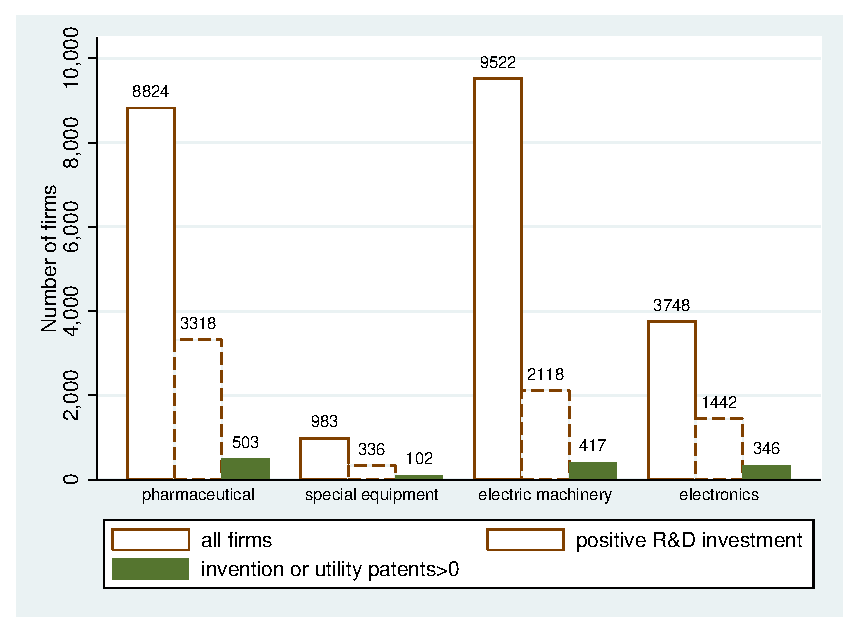
\includegraphics[width=0.8\textwidth]{FirmsCount.eps}
\par\end{centering}
\end{figure}
\par\end{center}

\section*{Appendix}

\subsection*{Math}

First let's write (\ref{nls}) as:
\[
r_{it}=\psi_{0}+\psi_{t}+\left(1+\theta\right)\left(\beta_{k}k_{it}+\beta_{a}a_{it}-\omega_{it}\right)
\]
Combining the expressions in (\ref{pi0(10)})-(\ref{pi}), we can
express the profit function as
\begin{align*}
\pi\left(\omega_{it},\,\bar{n}_{it},\,\bar{b}_{it},\,\bar{d}_{it}\right) & =-\frac{1}{\theta}\exp\left(\psi_{0}+\psi_{t}+\left(1+\theta\right)\left(\beta_{k}k_{it}+\beta_{a}a_{it}-\omega_{it}\right)\right)\\
 & +\eta_{0}\bar{n}_{it}+\eta_{1}\bar{b}_{it}
\end{align*}
Plugging (\ref{mk}) and (\ref{invp}) and (\ref{utip}) to the equation
above yields:
\begin{align*}
\pi\left(\omega_{it+1},\,\bar{n}_{it+1},\,\bar{b}_{it+1}|\omega_{it},\,rd_{it}\right) & =-\frac{1}{\theta}\exp\left\{ \begin{array}{c}
\psi_{0}+\psi_{t}+\left(1+\theta\right)\left(\beta_{k}k_{it}+\beta_{a}a_{it}-\rho_{1}\omega_{it}-\rho_{2}\omega_{it}^{2}\right)\\
-\left(1+\theta\right)\left(\rho_{0}+\alpha_{0}\rho_{4}+\alpha_{1}\rho_{5}\right)-\varepsilon_{it+1}
\end{array}\right\} \times\\
 & \exp\left\{ \left(\beta_{0}\rho_{4}+\beta_{1}\rho_{5}\right)rd_{it}\right\} \\
 & +\eta\left[\sum_{i=0}^{1}\alpha_{i}+\left(\sum_{i=0}^{1}\beta_{i}\right)rd_{it}\right]
\end{align*}
Note that $\int_{-\infty}^{+\infty}\exp\left(-\varepsilon\right)\frac{1}{\sqrt{2\pi}\sigma_{\varepsilon}}\exp\left(-\frac{\varepsilon^{2}}{2\sigma_{\varepsilon}^{2}}\right)d\varepsilon=\exp\left(\frac{\sigma_{\varepsilon}^{2}}{2}\right)$,
then if we denote 
\begin{align*}
\Xi\left(\Omega_{it}\right) & \equiv-\frac{1}{\theta}\exp\left\{ \begin{array}{c}
\psi_{0}+\psi_{t}+\left(1+\theta\right)\left(\beta_{k}k_{it}+\beta_{a}a_{it}-\rho_{1}\omega_{it}-\rho_{2}\omega_{it}^{2}-\rho_{3}\omega_{it}^{3}\right)\\
-\left(1+\theta\right)\left(\rho_{0}+\alpha_{0}\rho_{4}+\alpha_{1}\rho_{5}\right)+\frac{\sigma_{\varepsilon}^{2}}{2}
\end{array}\right\} \\
A & \equiv\beta_{0}\rho_{4}+\beta_{1}\rho_{5}
\end{align*}
which can be simplified as:
\[
\mathbb{E}_{t}\pi_{t+1}\left(\omega_{it+1},\,\bar{n}_{it+1},\,\bar{b}_{it+1}|\omega_{it},\,rd_{it}\right)=\Xi_{it}\exp\left(A\cdot rd_{it}\right)
\]


\subsection*{Computation}

\paragraph{Algorithm.}

Similar to \citet{Rust1987}, we can show that $EV\left(\Omega,\epsilon,\,rd\right)$
is a solution to following dynamic programming problem:
\begin{align}
EV\left(\Omega,\epsilon,\,rd\right) & =\int_{\Omega'}\int_{\epsilon'}\max_{rd'\geq0}\left\{ u\left(\Omega',\,\epsilon',\,rd'\right)+\delta EV\left(\Omega',\epsilon',\,rd'\right)\right\} p\left(d\Omega',\,d\epsilon'|\Omega,\,rd,\,\epsilon\right)
\end{align}
where $u\left(\Omega,\,\epsilon,\,rd\right)=\pi\left(\omega,\,rd_{-1}\right)-\mathbb{I}\left(rd>0\right)\exp\left(rd\right)\epsilon$.
By the conditional independence assumption on the transition density
of the controlled process given in \ref{CI}. This implies $EV\left(\Omega,\epsilon,\,rd\right)$
is independent of $\epsilon$ conditional on $rd$, so it can be expressed
as $EV\left(\Omega,\,rd\right)$. We define the social surplus function
associated with $p\left(\epsilon|\Omega\right)$ as:
\begin{align*}
S\left(\left\{ u\left(\Omega\right)+\delta EV\left(\Omega\right)\right\} |\Omega\right)\\
\equiv\int_{\epsilon}\max_{rd\geq0}\left\{ u\left(\Omega,\,\epsilon,\,rd\right)+\delta\mathbb{E}V\left(\Omega,\,rd\right)\right\} p\left(d\epsilon|\Omega\right)
\end{align*}
Then this function is the unique fixed point to a contraction mapping
$T_{\Theta}$, which is defined by:
\begin{equation}
T_{\Theta}\left(EV\left(\Omega,\,rd\right)\right)=\int_{\Omega'}S\left(\left\{ u\left(\Omega'\right)+\beta\mathbb{E}V\left(\Omega'\right)\right\} |\Omega'\right)p\left(d\Omega'|\Omega,\,rd\right)\label{vf_final}
\end{equation}
To solve this problem, I first approximate this problem by discretizing
the choice space. Specifically, the choice space is chosen to be 
\[
\mathcal{C}\equiv\left\{ x_{0},\,x_{1},\,x_{2},\,\cdots,\,x_{N}\right\} 
\]
where $x_{i}$ are non-negative grid points, $x_{0}=0$, and $x_{i-1}<x_{i}$,
for $i\geq1$. Therefore for $rd\in\mathcal{C}$, \ref{vf_final}
can be approximated by:
\begin{align*}
EV\left(\Omega,\,rd\right) & =\int_{\Omega'}S\left(\left\{ u\left(\Omega\right)+\delta EV\left(\Omega\right)\right\} |\Omega\right)p\left(d\Omega'|\Omega,\,rd\right)\\
 & =\int_{\Omega'}\int_{\epsilon}\max_{rd'\geq0}\left\{ u\left(\Omega,\,\epsilon,\,rd'\right)+\delta\mathbb{E}V\left(\Omega,\,rd'\right)\right\} p\left(d\epsilon|\Omega\right)p\left(d\Omega'|\Omega,\,rd\right)
\end{align*}
Denote $\Delta EV\left(\Omega,\,rd\right)\equiv EV\left(\Omega,\,rd\right)-EV\left(\Omega,0\right)$
and $\mathcal{C}_{1}\equiv\mathcal{C}\backslash\left\{ x_{0}\right\} $,
then the probability that a firm chooses not to invest in R\&D is
given by:
\begin{align}
\text{Pr}\left(rd=0|\Omega\right) & =\text{Pr}\left\{ \max_{rd\in\mathcal{C}_{1}}\left(\Delta EV\left(\Omega,\,rd\right)-\epsilon rd\right)\leq0\right\} \nonumber \\
 & =\text{Pr}\left\{ \epsilon\geq\max_{rd\in\mathcal{C}_{1}}\left(\frac{\Delta EV\left(\Omega,\,rd\right)}{rd}\right)\right\} \nonumber \\
 & =\exp\left\{ -\kappa_{-1}^{-1}\max_{rd\in\mathcal{C}_{1}}\left\{ \frac{\Delta EV\left(\Omega,\,rd\right)}{rd}\right\} \right\} \label{Pr(0|x)}
\end{align}

In this subsection, I list the steps for estimating the parameters
that match the R\&D choice in the dataset and predicted by the model. 

\paragraph{Implementation. }
\begin{enumerate}
\item Discretize the state variables and the choice set into grid points.\\
\textsl{Exogenous variables:} $\left(k_{it},\,a_{it},\,t,\,industry\right)$.
I treat them as exogenous variables that classify firm types. The
firm type is classified to be 100 values of capital stock, 4 values
of age, 6 values of year, and 4 2-digit industries, which gives me
$100\times4\times6\times4=8100$ types of firms.\\
\textsl{Endogenous variables:} $\left(\omega_{it},\,rd_{it-1}\right)$.
I discretize the state space into 100 grid points for productivity.
In the data I observe the log of R\&D expenditures lie between 0 and
12.382. I choose $x_{N}=15$, 20\% larger than the maximum value in
the dataset. I choose the interval between $x_{i+1}$ and $x_{i}$
to be $0.05$, so that $N=300$. Therefore I obtain a grid of 30,000
points.
\item Solving the value function using simulated method.\\
Starting from an initial guess for the parameters of interest: $\Theta_{0}$,
using iteration to solve the value function$EV\left(\Omega_{it},\,rd_{it}\right)$
and the conditional choice probability $\text{Pr}\left(rd_{it}=0|\Omega_{it}\right)$.\\
\textsl{Simulating the distribution of $\epsilon_{it}$:} Using initial
values of $\kappa_{0}^{s}$ and $\kappa_{0}^{m}$ to simulate two
distributions $\mathcal{E}_{0}^{0}$ and $\mathcal{E}_{0}^{1}$, where
\begin{align*}
\mathcal{E}_{0}^{0} & \sim\text{Exp}\left(\kappa_{0}^{s}\right)\\
\mathcal{E}_{0}^{1} & \sim\text{Exp}\left(\kappa_{0}^{m}\right)
\end{align*}
I use exponential random number generator to generate a vector of
$M=10000$ arguments to approximate the distribution. \\
\textsl{Solve $\mathbb{E}V\left(\Omega_{it},\,rd_{it}\right)$}: The
objective is a value function defined on the space of $\left(\omega_{it},\,rd_{it-1},\,rd_{it}\right)$,
which is a $60000$ (i.e., $200\times300$)-dimension vector. I compute
the social surplus function $S\left(\left\{ u\left(\Omega\right)+\delta EV\left(\Omega\right)\right\} |\Omega\right)$
using Monte Carlo method so that 
\begin{align*}
\int_{\epsilon}\max_{rd\geq0}\left\{ u\left(\omega_{it},\,rd_{-1},\,\epsilon,\,rd\right)+\delta\mathbb{E}V\left(\omega_{it},\,rd{}_{it-1},\,rd\right)\right\} p\left(d\epsilon|rd_{it}\right)\\
\thickapprox\frac{1}{M}\sum_{m=1}^{M}\max_{rd\in\mathcal{C}}\left\{ u\left(\omega_{it},\,rd_{it-1},\,\epsilon_{m},\,rd\right)+\delta\mathbb{E}V\left(\omega_{it},\,rd_{it-1},\,rd\right)\right\} \cdot\frac{\exp\left(-\epsilon_{m}/\kappa_{it}\right)}{\kappa_{it}}
\end{align*}
where $\epsilon_{m}$ is the $m$th point in the vector that approximate
the distribution of $\epsilon_{it}$. The transition matrix of productivity
is obtained using Tauchen method. For each level of R\&D expenditure
$rd\in\mathcal{C}$, I denote the transition matrix of productivity
to be $T_{rd}$. Then the iteration is as following:
\begin{align*}
\mathbb{E}V_{n+1}\left(\Omega_{it},\,rd\right) & =T_{rd}S\left(\left\{ u\left(\Omega_{it}\right)+\delta EV\left(\Omega_{it}\right)\right\} |\Omega_{it}\right)
\end{align*}
Under a given tolerance $tol$, the iteration stops when$\|\mathbb{E}V_{n+1}-\mathbb{E}V_{n}\|\leq tol$. 
\item Compute the maximum likelihood function.\\
\textsl{Compute the conditional probability $\text{Pr}\left(rd_{it}=0|\omega_{it},\,rd_{it-1}\right)$:}
I use the formula shown\textsl{ (\ref{Pr(0|x)}):}
\[
\text{Pr}\left(rd_{it}=0|\omega_{it},\,rd_{it-1}\right)=\exp\left\{ -\kappa_{it-1}^{-1}\max_{rd\in\mathcal{C}_{1}}\left\{ \frac{\Delta\mathbb{E}V\left(\omega_{it},\,rd_{it-1}\,rd\right)}{rd}\right\} \right\} 
\]
\textsl{Compute the LLF.} I plug (\ref{epsilon_diff}) and $\text{Pr}\left(rd_{it}=0|\omega_{it},\,rd_{it-1}\right)$
into (\ref{LLF}) to compute the LLF. 
\item To avoid the circumstance where the computed information matrix is
not positive semi-definite, I use BHHH algorithm to find the solution
to the minimization problem.
\end{enumerate}

\end{document}
